% Tikz script to create a PRISMA flowchart for a meta-analysis written by Gross, Wilson, & Wolak
% Title: “The fitness consequences of wildlife conservation translocations: A meta-analysis” 
% Date: 230205

\documentclass{article}
\usepackage[utf8]{inputenc}
\usepackage{tikz}
\usepackage{pdflscape}

\title{flow}
\author{Iwo Gross}
\date{December 2022}
\usetikzlibrary{shapes.geometric, arrows}


\tikzstyle{output} = [rectangle, text centered, draw=black,thick, fill=green!15, minimum width=3cm, minimum height=1cm]
\tikzstyle{data} = [rectangle, text centered, draw=black,thick, fill=orange!15, minimum width=2cm, minimum height=1cm]
\tikzstyle{data2} = [rectangle, text centered, draw=black,thick, fill=blue!15, minimum width=2cm, minimum height=1cm]
\tikzstyle{remove} = [rectangle, rounded corners, text centered, draw=black,thick, fill=orange!15, minimum width=2cm, minimum height=1cm]
\tikzstyle{remove2} = [rectangle, rounded corners, text centered, draw=black,thick, fill=blue!15, minimum width=2cm, minimum height=1cm]
\tikzstyle{function} = [rectangle, text centered, draw=black,thick, fill=black!15, minimum width=3cm, minimum height=1cm]
\tikzstyle{arrow} = [thick, ->, >=stealth]

\begin{document}
\begin{landscape}
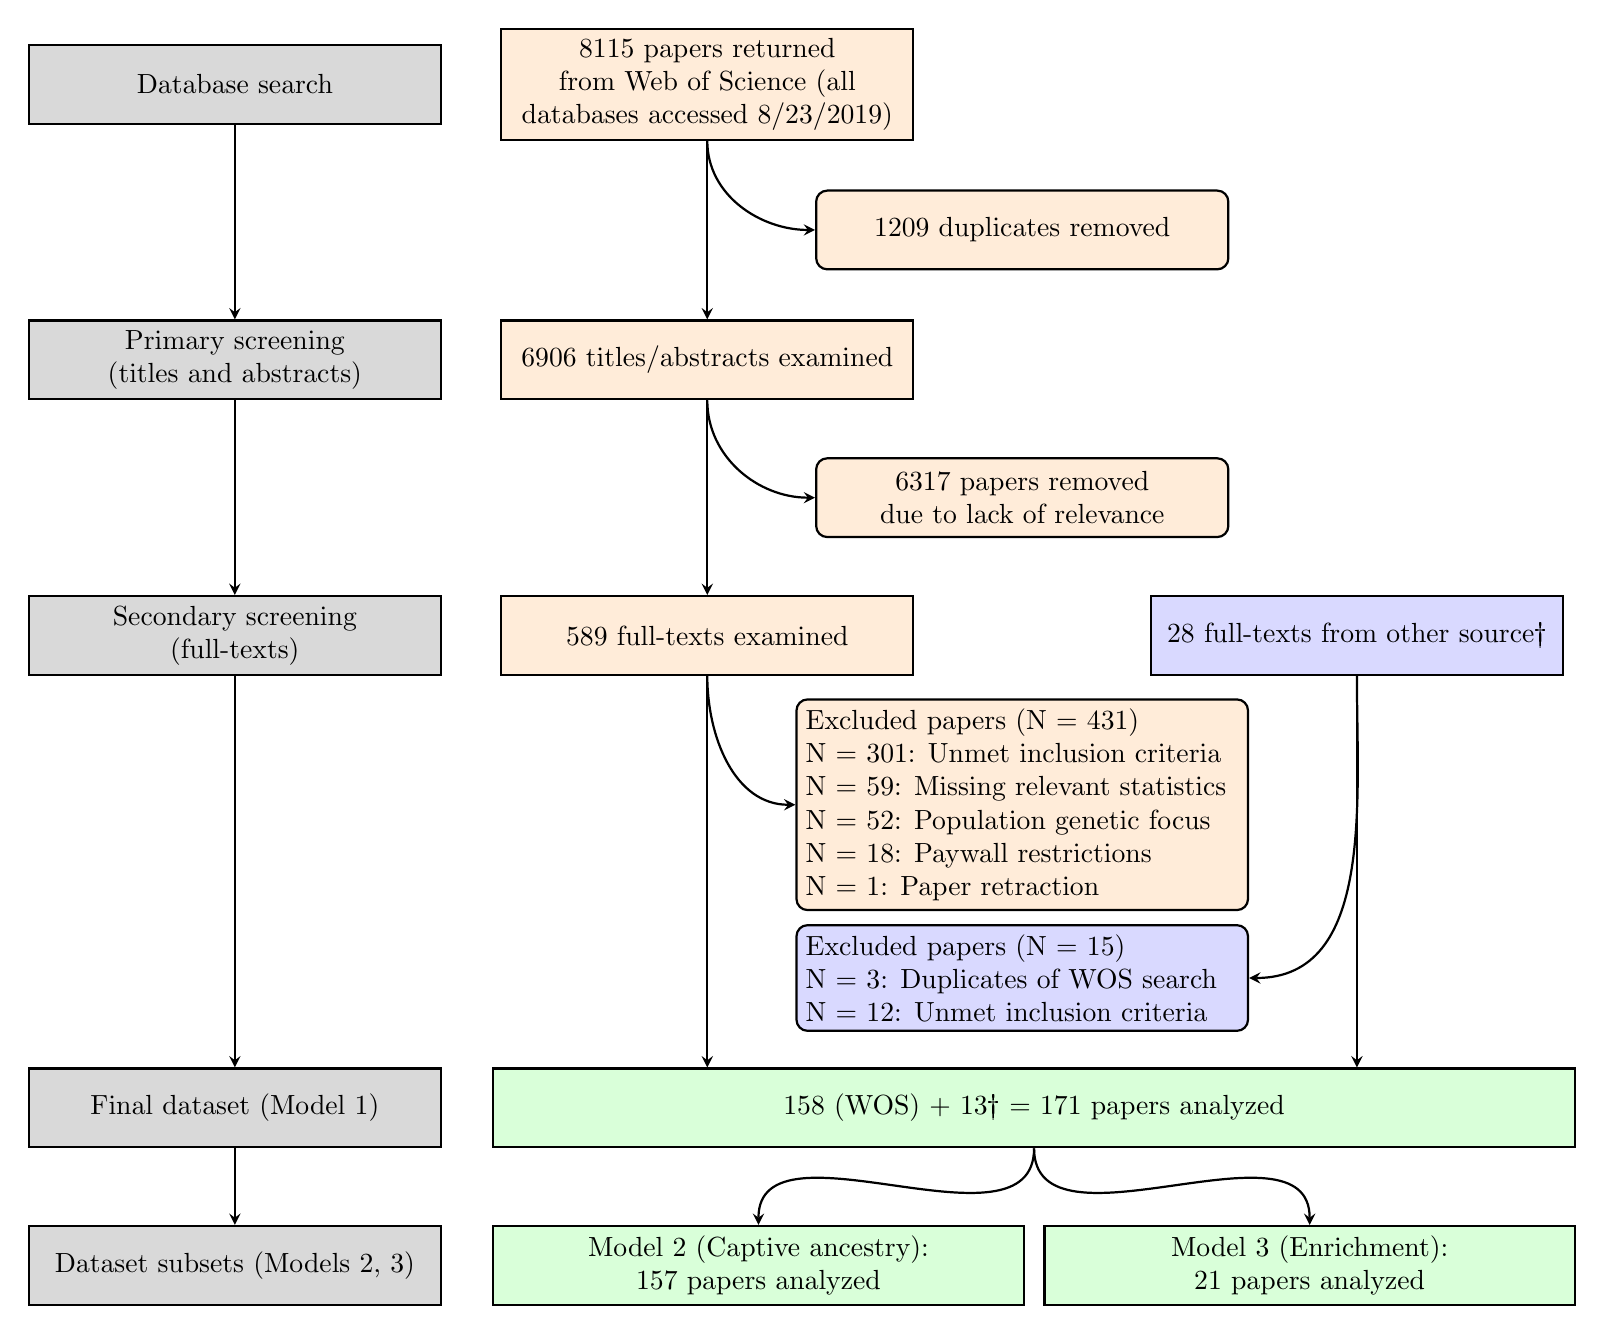
\begin{tikzpicture}[node distance=2cm]


\node (query) [data, text width = 5cm] {8115 papers returned from Web of Science (all databases accessed 8/23/2019)};
\node (screen1) [data, text width = 5cm, below of=query, yshift=-1.5cm] {6906 titles/abstracts examined};
\node (screen2) [data, text width = 5cm, below of=screen1, yshift=-1.5cm] {589 full-texts examined};
\node (stuparyk) [data2, text width = 5cm, right of=screen2, xshift=6.25cm] {28 full-texts from other source{\textdagger}};
\node (final) [output, text width = 13.5cm, below of=screen2, xshift = 4.15cm, yshift=-4cm] {158 (WOS) + 13{\textdagger} = 171 papers analyzed};
\node (subset1) [output, text width = 6.5cm, below of=final, xshift = -3.5cm] {Model 2 (Captive ancestry):\\ 157 papers analyzed};
\node (subset2) [output, text width = 6.5cm, below of=final, xshift = 3.5cm] {Model 3 (Enrichment):\\ 21 papers analyzed};
\node (remove1) [remove, text width = 5cm, right of=query, xshift =2cm, yshift=-1.85cm] {1209 duplicates removed};
\node (remove3) [remove, text width = 5cm, right of=screen1, xshift =2cm, yshift=-1.75cm] {6317 papers removed due to lack of relevance};
\node (remove4) [remove, text width = 5.5cm, right of=screen2, xshift =2cm, yshift=-2.15cm, align=flush left] {Excluded papers (N = 431) \\N = 301: Unmet inclusion criteria \\N = 59: Missing relevant statistics \\N = 52: Population genetic focus \\N = 18: Paywall restrictions \\N = 1: Paper retraction};
\node (remove5) [remove2, text width = 5.5cm, right of=screen2, xshift =2cm, yshift=-4.35cm, align=flush left] {Excluded papers (N = 15) \\ N = 3: Duplicates of WOS search\\ N = 12: Unmet inclusion criteria};

\node (func1) [function, text width = 5cm, left of =query, xshift = -4cm] {Database search};
\node (func2) [function, text width = 5cm, below of=func1, yshift=-1.5cm] {Primary screening\\(titles and abstracts)};
\node (func3) [function, text width = 5cm, below of=func2, yshift=-1.5cm] {Secondary screening\\(full-texts)};
\node (func4) [function, text width = 5cm, below of=func3, yshift=-4cm] {Final dataset (Model 1)};
\node (func5) [function, text width = 5cm, below of=func4] {Dataset subsets (Models 2, 3)};

\draw [arrow] (query) -- (screen1);
\draw [arrow] (screen1) -- (screen2);
\draw [arrow] (screen2) -- ([xshift=-4.15cm]final.north);
;
\draw [arrow] (query) to [out=270,in=180] (remove1);

\draw [arrow] (screen1) to [out=270,in=180] (remove3);
\draw [arrow] (screen2) to [out=270,in=180] (remove4);
\draw [arrow] (stuparyk) to [out=270,in=0] (remove5);
\draw [arrow] (final) to [out=270,in=90] (subset1);
\draw [arrow] (final) to [out=270,in=90] (subset2);
\draw [arrow] (stuparyk) -- ([xshift=4.1cm]final.north);

\draw [arrow] (func1) -- (func2);
\draw [arrow] (func2) -- (func3);
\draw [arrow] (func3) -- (func4);
\draw [arrow] (func4) -- (func5);



\end{tikzpicture}
\end{landscape}
\end{document}
